\documentclass[../../thesis.tex]{subfiles}

\begin{document}

\section{Topologies}\label{sec:topologies}
For our tests, we used three UAM network topologies, first introduced in \cite{pelegrin-2023} and depicted in Figure \ref{pic:topologies}.  
We adopted the same method for generating these networks and utilized the 
original code, 
%capire se mantenere la seguente riga
applying minor fixes due to changes in the Python version.
A detailed explanation of the instance generation process is provided in Section \ref{sec:generationInstance}.  

%Each path is mono-directional, and path changes are only allowed at predetermined points.  
The figure also illustrates the travel times (based on a default speed) and the vertiports, represented by $\times$.  
Vertiports are the only nodes where a collaborative flight can depart or arrive.  

\begin{enumerate}
    \item \textbf{Grid}: Shown in Figure \ref{fig:grid}, this topology consists of 8 vertiports arranged in a grid layout.
    \item \textbf{Airport}: Represented in Figure \ref{fig:airport}, this topology includes 4 vertiports, interconnected through a central airport via a fifth vertiport.
    \item \textbf{Metroplex}: Depicted in Figure \ref{fig:metroplex}, this topology features two densely connected regions, with 3 and 6 vertiports respectively, linked by a single corridor.
\end{enumerate}

The graphs are directed, and intersections between two tracks are modeled as shown in Figure \ref{fig:crossingTrack}.  
To allow for greater flexibility in speed changes, additional "waypoint" nodes are inserted along the arcs at intervals of one minute of travel time at default speed.

\begin{figure}
\centering
\begin{subfigure}{0.45\textwidth}
    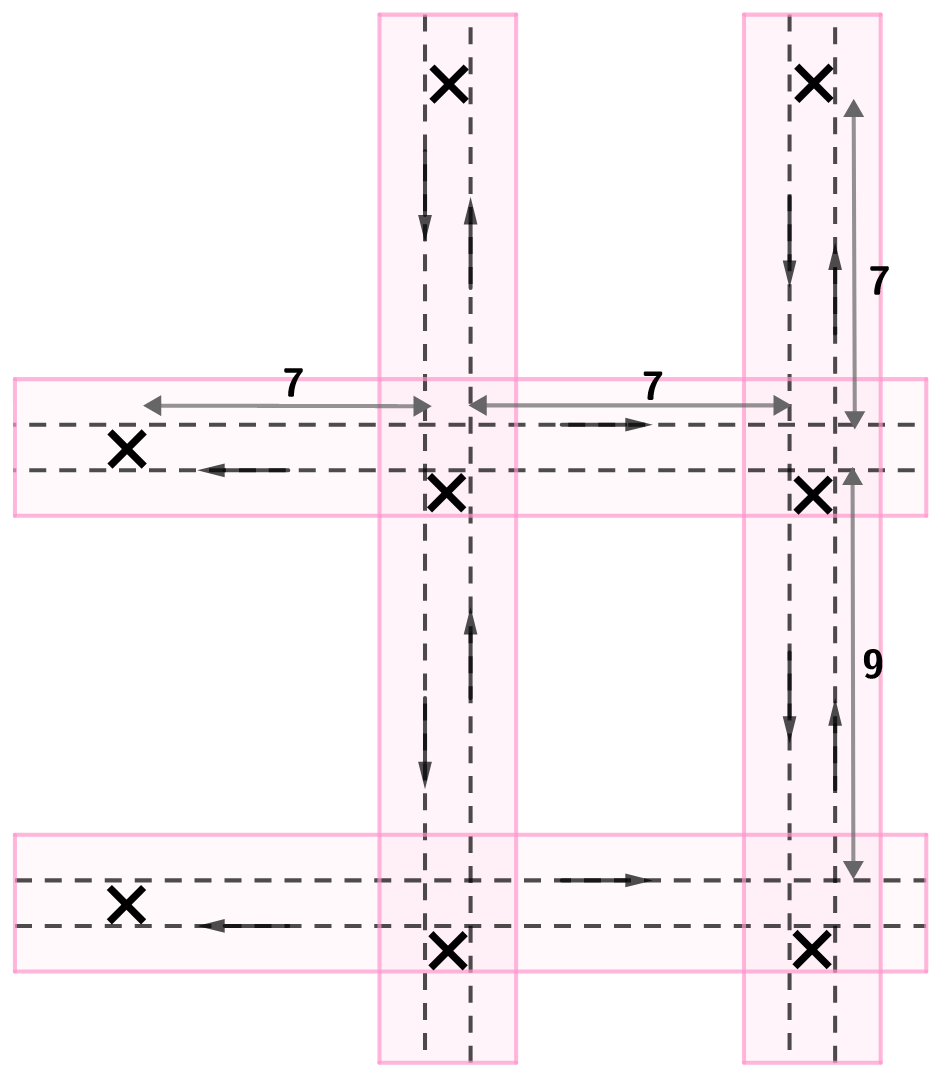
\includegraphics[width=\textwidth]{thesis/picture/topologies/net1.png}
    \caption{Grid topology}
    \label{fig:grid}
\end{subfigure}
\hfill
\begin{subfigure}{0.45\textwidth}
    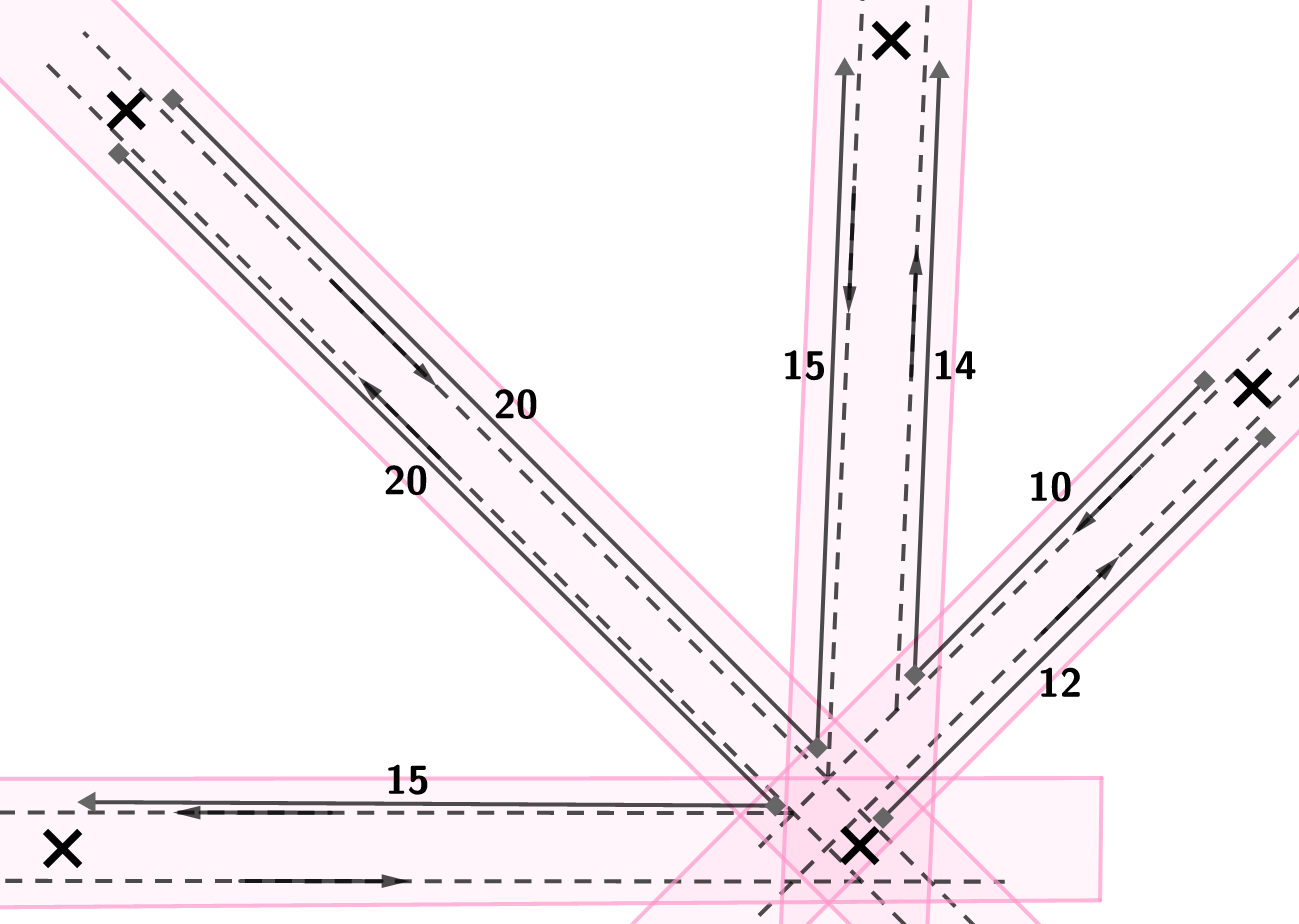
\includegraphics[width=\textwidth]{thesis/picture/topologies/net2.png}
    \caption{Airport topology}
    \label{fig:airport}
\end{subfigure}
\hfill
\begin{subfigure}{0.7\textwidth}
    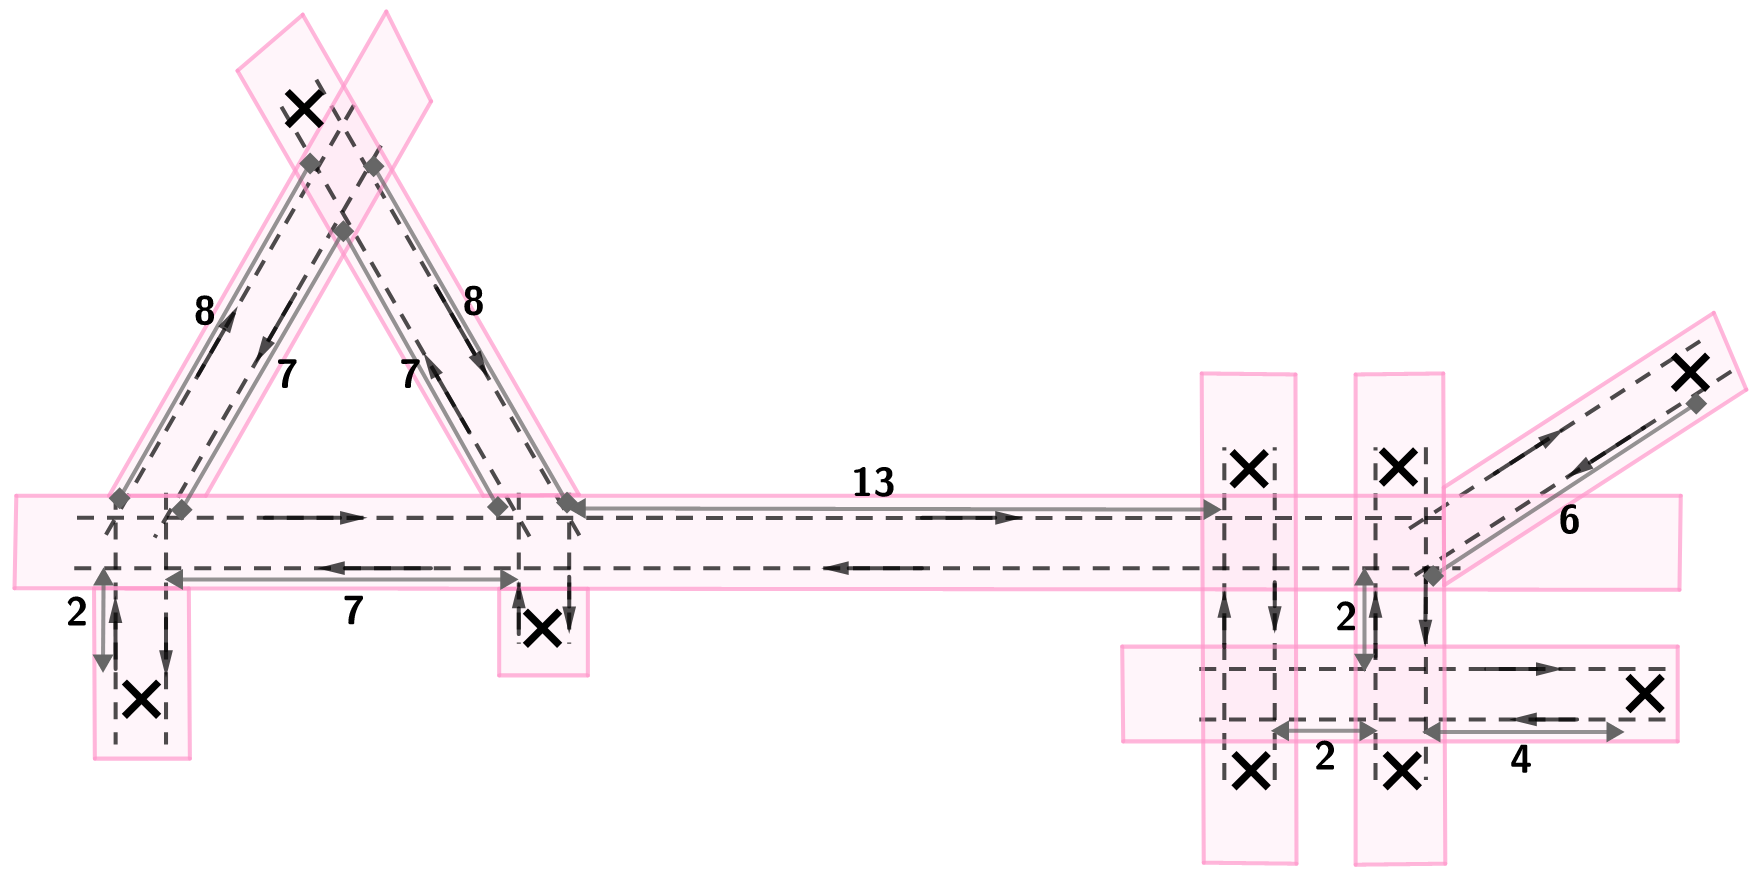
\includegraphics[width=\textwidth]{thesis/picture/topologies/net3.png}
    \caption{Metroplex topology}
    \label{fig:metroplex}
\end{subfigure}
        
\caption{Track network topologies}
\label{pic:topologies}
\end{figure}


\begin{figure}
    \centering
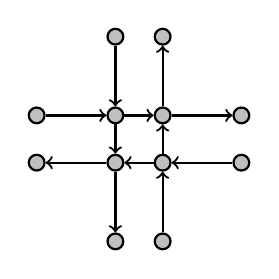
\begin{tikzpicture}[node distance={10mm}, thick, main/.style = {draw, circle, fill=gray!50},minimum size=2mm,inner sep=0pt] 
\node[main] (1) {}; 
\node[main] (2)  [right of=1][node distance={6mm}] {}; 
\node[main] (3)  [below of=2][node distance={6mm}] {}; 
\node[main] (4)  [left  of=3][node distance={6mm}] {}; 
\node[main] (5)  [left  of=1] {}; 
\node[main] (6)  [above of=1] {}; 
\node[main] (7)  [right of=2] {}; 
\node[main] (8)  [above of=2] {}; 
\node[main] (9)  [right of=3] {}; 
\node[main] (10) [below of=3] {}; 
\node[main] (11) [left  of=4] {}; 
\node[main] (12) [below of=4] {}; 

\draw[->] (1) -- (2); 
\draw[->] (1) -- (4);
\draw[->] (2) -- (7); 
\draw[->] (2) -- (8); 
\draw[->] (3) -- (2); 
\draw[->] (3) -- (4); 
\draw[->] (4) -- (11); 
\draw[->] (4) -- (12); 
\draw[->] (5) -- (1); 
\draw[->] (6) -- (1); 
\draw[->] (9) -- (3); 
\draw[->] (10) -- (3);  

\end{tikzpicture} 

    \caption{Modeling crossing track with directed graph}
    \label{fig:crossingTrack}
\end{figure}
\end{document}